\section{Feed-Forward Neural Networks}
A feed-forward neural network is a function $h: \mathcal{X} \mapsto \mathcal{Y}$. To understand how it works, it's instructive to look at each part of its name in isolation.
\\\\
$h$ is called a \textbf{network} because it's a composition of $L$ \textbf{layers} of other functions $f^{(l)}$. Each function $f^{(l)}$ receives input from $f^{(l-1)}$. For example if $L = 2$, then $h(\mathbf{x}) = f^{(2)}(f^{(1)}(\mathbf{x}))$. Each $f^{(l)}$ outputs a vector $\mathbf{x}^{(l)}$ of dimension $d^{(l)}$.  We denote the input to $f^{(1)}$ as $\mathbf{x}^{(0)}$ which is identical to the input vector $\mathbf{x}$ with an added \textbf{bias} component as described later in this section. The dimensionality of these vectors determine the \textbf{width} of the network. The number of layers $L$ is called the \textbf{depth} of the network. $f^{(L)}$ is called the \textbf{output layer}. The remaining functions $f^{(1)}$ to $f^{(L-1)}$ are called \textbf{hidden layers}. 
\\\\
The functions $f^{(1)}$ to $f^{(L)}$ are ordered by their index $l$ such that the index of the layers increase as we move from the input to the output layer. $h$ is called a \textbf{feed-forward} network because each $f^{(l)}$ can receive input only from functions $f^{(i)}$ if $l > i$. In other words, it's not possible for a function $f^{(l)}$ to feed its own output into itself, or any other function that it receives input from.
\\\\
Finally, $h$ is called a \textbf{neural} network since its design is loosely based on neurons in the brain \citep{goodfellow16}. Each component $x_i$ of the vector $\mathbf{x}^{(l)}$ can be seen as the output of a unit similar to a neuron. Each unit in layer $l$ receives input from units in layer $l-1$. The output $x^{(l-1)}_i$ of unit $i$ in layer $l-1$ is multiplied by a weight $w^{(l)}_{ij}$ that gives the strength of the connection between unit $i$ in $l-1$ and unit $j$ in $l$. Unit $j$ sums all of the input it receives from units in layer $l-1$ to obtain its \textbf{activation} $a^{(l)}_j = \sum_{i=0}^{d^{(l-1)}} w^{(l)}_{ij}x^{(l-1)}_{i}$. To compute its output $x^{(l)}_j$, it applies an \textbf{activation function} $\sigma(a^{(l)}_j)$ to the sum of its weighted input.

Activation functions model the behavior of biological neurons by outputting a signal only when the activation is above a certain threshold. To make it possible to learn this threshold for each unit using the same activation function, we introduce a special \textbf{bias} unit that always outputs 1. The index of the bias unit in layer $l$ is 0 by convention. Figure \ref{connection}. shows how a unit $j$ computes its output $x^{(l)}_j$ by combining the outputs of units in layer $l-1$.

\tikzstyle{neuron}=[circle,draw,minimum size=20pt,inner sep=0pt]
\tikzstyle{summation} = [square, minimum size=20pt,inner sep=0pt]
\tikzstyle{edge} = [draw,thick,-]
\tikzstyle{weight} = [font=\small]

\begin{figure}[h]
	\centering
	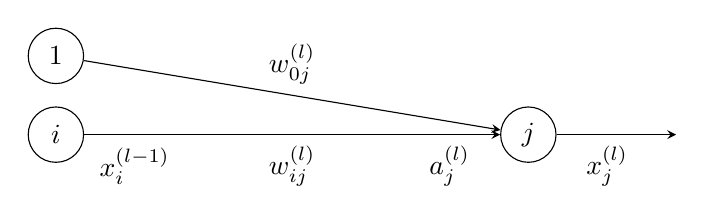
\begin{tikzpicture}[->, >=stealth, swap]
			\node [neuron] (sigma1) at (0,0) {$i$};
			\node [neuron] (sigma2) at (6,0) {$j$};
			\node [neuron] (bias1) at (0,1) {$1$};
			\node []       (z1)      at (1,-.4) {$x^{(l-1)}_i$};
			\node []       (w)     at (3,-.4) {$w^{(l)}_{ij}$};
			\node []       (w)     at (3,.9) {$w^{(l)}_{0j}$};
			\node []       (aw)   at (5,-.4) {$a^{(l)}_j$};
			\node []	   (empty) at (8,0) {};
			\node []       (z2)    at (7,-.4) {$x^{(l)}_j$};
		
			\draw (sigma1) edge (sigma2);
			\draw (sigma2) edge (empty);
			\draw (bias1) edge (sigma2);
	\end{tikzpicture}
	\caption{A visual representation of the connections between unit $i$ in layer $l-1$, the bias unit in $l-1$, and unit $j$ in layer $l$. The connection strength between these units is given by the weight $w^{(l)}_{ij}$ between $i$ and $j$, and $w^{(l)}_{0j}$ between the bias unit and $j$. The activation $a^{(l)}_j$ at unit $j$ is computed by $a^{(l)}_j = w^{(l)}_{ij}x^{(l)}_i + w^{(l)}_0$. The output $x^{(l)}_j$ of unit $j$ is given by $x^{(l)}_j = \sigma(a^{(l)}_j)$}
	\label{connection}
\end{figure}
\noindent
Keeping track of the indices $l$, $i$ and $j$ quickly becomes confusing. By collecting all of the weights of connections going into unit $j$ in layer $l$ in a vector $\mathbf{w}^{(l)}_j$, the activation at unit $j$ can be computed as a dot product $a^{(l)}_j = {\mathbf{w}^{(l)}_j} \cdot \mathbf{x}^{(l-1)}$. Moreover, we can compute the entire vector $\mathbf{a}^{(l)}$ of activations at layer $l$, by organising the weight vectors $\mathbf{w}^{(l)}_j$ in a matrix $\mathbf{W}^{(l)} = \begin{bmatrix} \mathbf{w}^{(l)}_1 & \dots & \mathbf{w}^{(l)}_{d^{(l)}} \end{bmatrix}^T$, which leads to $\mathbf{a}^{(l)} = \mathbf{W}^{(l)}\mathbf{x}^{(l-1)}$.
\\\\
By gathering the weights in matrices $\mathbf{W}^{(l)}$, we have simplified our view of $h$ into a composition of matrix-vector products and element-wise application of activation functions. Figure \ref{neural_network} shows the parallel views of neural networks as networks of units and matrix-vector operations.
\\\\
We now have all the components we need to specify $\mathcal{H}$ as a set of neural networks. The set is defined by the depth of the networks $L$, the number of units in each layer $d_l$ and the activation function $\sigma$.
For a particular $L$, $d_l$, and $\sigma$, each $h \in \mathcal{H}$ corresponds exactly to a unique assignment of real numbers to all of its weights. We can make the dependence of $h$ on its weights explicit by defining a vector $\mathbf{w} = \begin{bmatrix} w^{(1)}_{ij} & \dots & w^{(L)}_{ij}\end{bmatrix}$ and writing $h(\mathbf{x}, \mathbf{w})$ which means \textit{the function $h$ parameterised by the weight vector $\mathbf{w}$}. In practice, it's common to use different activation functions at different layers of the network. In the next section we discuss how to choose these activation functions.
\begin{figure}[h]
	\centering
	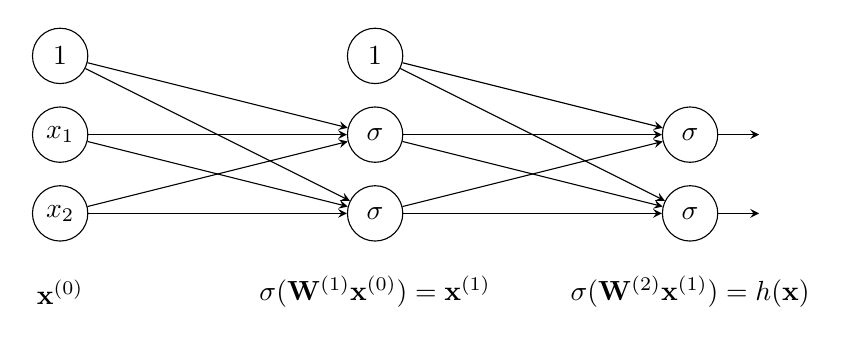
\begin{tikzpicture}[->, >=stealth, swap]
		\node [neuron] (bias0)   at (0, 2)  {1};
		\node [neuron] (x1)      at (0, 1)  {$x_1$};
		\node [neuron] (x2)      at (0, 0)  {$x_2$};
		\node []       (x)       at (0,-1)  {$\mathbf{x}^{(0)}$};
		\node [neuron] (bias1)   at (4, 2)  {1}; 
		\node [neuron] (sigma11) at (4, 1)  {$\sigma$};
		\node [neuron] (sigma12) at (4, 0)  {$\sigma$};
		\node []       (layer1)  at (4,-1)  {$\sigma(\mathbf{W}^{(1)} \mathbf{x}^{(0)}) = \mathbf{x}^{(1)}$};
		\node [neuron] (sigma21) at (8, 1)  {$\sigma$};
		\node [neuron] (sigma22) at (8, 0)  {$\sigma$};
		\node []       (layer2)  at (8,-1)  {$\sigma(\mathbf{W}^{(2)} \mathbf{x}^{(1)}) = h(\mathbf{x})$};
		\node []	   (empty1)  at (9, 1) {};
		\node []       (empty2)  at (9, 0) {};   
		
		
		\draw (bias0)   edge (sigma11);
		\draw (x1)      edge (sigma11);
		\draw (x2)      edge (sigma11);
		\draw (bias0)   edge (sigma12);
		\draw (x1)      edge (sigma12);
		\draw (x2)      edge (sigma12);
		\draw (bias1)   edge (sigma21);
		\draw (sigma11) edge (sigma21);
		\draw (sigma12) edge (sigma21);
		\draw (bias1)   edge (sigma22);
		\draw (sigma11) edge (sigma22);
		\draw (sigma12) edge (sigma22);
		\draw (sigma21) edge (empty1);
		\draw (sigma22) edge (empty2);
	\end{tikzpicture}
	\caption{A visual representation of $h = f_2(f_1(\mathbf{x}^{(0)}))$. The activation at each layer $\mathbf{a}^{(l)}$ is computed by $\mathbf{W}^{(l)}\mathbf{x}^{(l-1)}$. The output at each layer is computed by element-wise application of the activation function of $\sigma(\mathbf{a}^{(l)})$.}
	\label{neural_network}
\end{figure}

\subsection{Activation Functions}
\label{activation_functions}
Activation functions mimic the behaviour of neurons in the brain. A neuron emits a signal when the combined input it receives from other neurons exceeds a certain threshold. Activation functions achieve this by a variation of the step function, where an activation signal $a^{(l)}_j$ below the threshold is mapped to a value near zero and an activation signal above the threshold is mapped to a value greater than zero. From a mathematical perspective the role of activation functions is to introduce non-linearity in $h$ which allows $\mathcal{H}$ to model a larger class of functions \citep{goodfellow16}.
\\\\
Many networks use \textbf{sigmoidal} activation functions such as the classical sigmoid function $\sigma(a) = 1/(1 + \me^{-a})$. These functions have the advantage of being differentiable everywhere. As we will see in section \ref{learningAlgorithm}, differential calculus is the fundamental tool for finding a good $h \in \mathcal{H}$ which makes differentiability a desirable quality. One drawback of sigmoidal activation functions is that their derivates are small as seen in figure \ref{sigmoid}. As we will see in section \ref{learningAlgorithm}, neural networks are trained by multiplying chains of derivatives. When these derivatives are smaller than 1, the magnitude of the derivative shrinks in the length of the chain of terms which can make learning from $\mathcal{D}$ extremely slow.
\begin{figure}
	\centering
	%% Creator: Matplotlib, PGF backend
%%
%% To include the figure in your LaTeX document, write
%%   \input{<filename>.pgf}
%%
%% Make sure the required packages are loaded in your preamble
%%   \usepackage{pgf}
%%
%% Figures using additional raster images can only be included by \input if
%% they are in the same directory as the main LaTeX file. For loading figures
%% from other directories you can use the `import` package
%%   \usepackage{import}
%% and then include the figures with
%%   \import{<path to file>}{<filename>.pgf}
%%
%% Matplotlib used the following preamble
%%   \usepackage{fontspec}
%%   \setmainfont{Palatino}
%%   \setsansfont{Lucida Grande}
%%   \setmonofont{Andale Mono}
%%
\begingroup%
\makeatletter%
\begin{pgfpicture}%
\pgfpathrectangle{\pgfpointorigin}{\pgfqpoint{4.614828in}{3.237168in}}%
\pgfusepath{use as bounding box, clip}%
\begin{pgfscope}%
\pgfsetbuttcap%
\pgfsetmiterjoin%
\definecolor{currentfill}{rgb}{1.000000,1.000000,1.000000}%
\pgfsetfillcolor{currentfill}%
\pgfsetlinewidth{0.000000pt}%
\definecolor{currentstroke}{rgb}{1.000000,1.000000,1.000000}%
\pgfsetstrokecolor{currentstroke}%
\pgfsetdash{}{0pt}%
\pgfpathmoveto{\pgfqpoint{0.000000in}{-0.000000in}}%
\pgfpathlineto{\pgfqpoint{4.614828in}{-0.000000in}}%
\pgfpathlineto{\pgfqpoint{4.614828in}{3.237168in}}%
\pgfpathlineto{\pgfqpoint{0.000000in}{3.237168in}}%
\pgfpathclose%
\pgfusepath{fill}%
\end{pgfscope}%
\begin{pgfscope}%
\pgfsetbuttcap%
\pgfsetmiterjoin%
\definecolor{currentfill}{rgb}{1.000000,1.000000,1.000000}%
\pgfsetfillcolor{currentfill}%
\pgfsetlinewidth{0.000000pt}%
\definecolor{currentstroke}{rgb}{0.000000,0.000000,0.000000}%
\pgfsetstrokecolor{currentstroke}%
\pgfsetstrokeopacity{0.000000}%
\pgfsetdash{}{0pt}%
\pgfpathmoveto{\pgfqpoint{0.074056in}{0.375732in}}%
\pgfpathlineto{\pgfqpoint{4.559273in}{0.375732in}}%
\pgfpathlineto{\pgfqpoint{4.559273in}{3.237168in}}%
\pgfpathlineto{\pgfqpoint{0.074056in}{3.237168in}}%
\pgfpathclose%
\pgfusepath{fill}%
\end{pgfscope}%
\begin{pgfscope}%
\pgfpathrectangle{\pgfqpoint{0.074056in}{0.375732in}}{\pgfqpoint{4.485217in}{2.861436in}} %
\pgfusepath{clip}%
\pgfsetrectcap%
\pgfsetroundjoin%
\pgfsetlinewidth{1.003750pt}%
\definecolor{currentstroke}{rgb}{0.000000,0.000000,1.000000}%
\pgfsetstrokecolor{currentstroke}%
\pgfsetdash{}{0pt}%
\pgfpathmoveto{\pgfqpoint{0.074056in}{0.375850in}}%
\pgfpathlineto{\pgfqpoint{0.522578in}{0.376604in}}%
\pgfpathlineto{\pgfqpoint{0.724412in}{0.377877in}}%
\pgfpathlineto{\pgfqpoint{0.858969in}{0.379637in}}%
\pgfpathlineto{\pgfqpoint{0.971099in}{0.382164in}}%
\pgfpathlineto{\pgfqpoint{1.060804in}{0.385316in}}%
\pgfpathlineto{\pgfqpoint{1.128082in}{0.388652in}}%
\pgfpathlineto{\pgfqpoint{1.195360in}{0.393142in}}%
\pgfpathlineto{\pgfqpoint{1.240212in}{0.396965in}}%
\pgfpathlineto{\pgfqpoint{1.285064in}{0.401620in}}%
\pgfpathlineto{\pgfqpoint{1.329917in}{0.407282in}}%
\pgfpathlineto{\pgfqpoint{1.374769in}{0.414164in}}%
\pgfpathlineto{\pgfqpoint{1.419621in}{0.422520in}}%
\pgfpathlineto{\pgfqpoint{1.464473in}{0.432652in}}%
\pgfpathlineto{\pgfqpoint{1.486899in}{0.438494in}}%
\pgfpathlineto{\pgfqpoint{1.509325in}{0.444919in}}%
\pgfpathlineto{\pgfqpoint{1.531751in}{0.451982in}}%
\pgfpathlineto{\pgfqpoint{1.554177in}{0.459742in}}%
\pgfpathlineto{\pgfqpoint{1.576604in}{0.468263in}}%
\pgfpathlineto{\pgfqpoint{1.599030in}{0.477614in}}%
\pgfpathlineto{\pgfqpoint{1.621456in}{0.487867in}}%
\pgfpathlineto{\pgfqpoint{1.643882in}{0.499101in}}%
\pgfpathlineto{\pgfqpoint{1.666308in}{0.511399in}}%
\pgfpathlineto{\pgfqpoint{1.688734in}{0.524850in}}%
\pgfpathlineto{\pgfqpoint{1.711160in}{0.539545in}}%
\pgfpathlineto{\pgfqpoint{1.733586in}{0.555582in}}%
\pgfpathlineto{\pgfqpoint{1.756012in}{0.573062in}}%
\pgfpathlineto{\pgfqpoint{1.778438in}{0.592090in}}%
\pgfpathlineto{\pgfqpoint{1.800864in}{0.612771in}}%
\pgfpathlineto{\pgfqpoint{1.823290in}{0.635213in}}%
\pgfpathlineto{\pgfqpoint{1.845717in}{0.659526in}}%
\pgfpathlineto{\pgfqpoint{1.868143in}{0.685815in}}%
\pgfpathlineto{\pgfqpoint{1.890569in}{0.714184in}}%
\pgfpathlineto{\pgfqpoint{1.912995in}{0.744730in}}%
\pgfpathlineto{\pgfqpoint{1.935421in}{0.777543in}}%
\pgfpathlineto{\pgfqpoint{1.957847in}{0.812703in}}%
\pgfpathlineto{\pgfqpoint{1.980273in}{0.850276in}}%
\pgfpathlineto{\pgfqpoint{2.002699in}{0.890312in}}%
\pgfpathlineto{\pgfqpoint{2.025125in}{0.932841in}}%
\pgfpathlineto{\pgfqpoint{2.047551in}{0.977870in}}%
\pgfpathlineto{\pgfqpoint{2.069977in}{1.025382in}}%
\pgfpathlineto{\pgfqpoint{2.092403in}{1.075331in}}%
\pgfpathlineto{\pgfqpoint{2.114830in}{1.127641in}}%
\pgfpathlineto{\pgfqpoint{2.137256in}{1.182203in}}%
\pgfpathlineto{\pgfqpoint{2.159682in}{1.238877in}}%
\pgfpathlineto{\pgfqpoint{2.182108in}{1.297488in}}%
\pgfpathlineto{\pgfqpoint{2.226960in}{1.419668in}}%
\pgfpathlineto{\pgfqpoint{2.271812in}{1.546751in}}%
\pgfpathlineto{\pgfqpoint{2.406369in}{1.933102in}}%
\pgfpathlineto{\pgfqpoint{2.451221in}{2.055281in}}%
\pgfpathlineto{\pgfqpoint{2.473647in}{2.113893in}}%
\pgfpathlineto{\pgfqpoint{2.496073in}{2.170566in}}%
\pgfpathlineto{\pgfqpoint{2.518499in}{2.225129in}}%
\pgfpathlineto{\pgfqpoint{2.540925in}{2.277439in}}%
\pgfpathlineto{\pgfqpoint{2.563351in}{2.327388in}}%
\pgfpathlineto{\pgfqpoint{2.585777in}{2.374900in}}%
\pgfpathlineto{\pgfqpoint{2.608203in}{2.419929in}}%
\pgfpathlineto{\pgfqpoint{2.630629in}{2.462457in}}%
\pgfpathlineto{\pgfqpoint{2.653056in}{2.502493in}}%
\pgfpathlineto{\pgfqpoint{2.675482in}{2.540066in}}%
\pgfpathlineto{\pgfqpoint{2.697908in}{2.575226in}}%
\pgfpathlineto{\pgfqpoint{2.720334in}{2.608040in}}%
\pgfpathlineto{\pgfqpoint{2.742760in}{2.638586in}}%
\pgfpathlineto{\pgfqpoint{2.765186in}{2.666954in}}%
\pgfpathlineto{\pgfqpoint{2.787612in}{2.693243in}}%
\pgfpathlineto{\pgfqpoint{2.810038in}{2.717556in}}%
\pgfpathlineto{\pgfqpoint{2.832464in}{2.739999in}}%
\pgfpathlineto{\pgfqpoint{2.854890in}{2.760680in}}%
\pgfpathlineto{\pgfqpoint{2.877316in}{2.779707in}}%
\pgfpathlineto{\pgfqpoint{2.899742in}{2.797187in}}%
\pgfpathlineto{\pgfqpoint{2.922168in}{2.813225in}}%
\pgfpathlineto{\pgfqpoint{2.944595in}{2.827920in}}%
\pgfpathlineto{\pgfqpoint{2.967021in}{2.841370in}}%
\pgfpathlineto{\pgfqpoint{2.989447in}{2.853668in}}%
\pgfpathlineto{\pgfqpoint{3.011873in}{2.864902in}}%
\pgfpathlineto{\pgfqpoint{3.034299in}{2.875156in}}%
\pgfpathlineto{\pgfqpoint{3.056725in}{2.884506in}}%
\pgfpathlineto{\pgfqpoint{3.079151in}{2.893027in}}%
\pgfpathlineto{\pgfqpoint{3.101577in}{2.900787in}}%
\pgfpathlineto{\pgfqpoint{3.124003in}{2.907851in}}%
\pgfpathlineto{\pgfqpoint{3.146429in}{2.914276in}}%
\pgfpathlineto{\pgfqpoint{3.191281in}{2.925427in}}%
\pgfpathlineto{\pgfqpoint{3.236134in}{2.934630in}}%
\pgfpathlineto{\pgfqpoint{3.280986in}{2.942214in}}%
\pgfpathlineto{\pgfqpoint{3.325838in}{2.948457in}}%
\pgfpathlineto{\pgfqpoint{3.370690in}{2.953591in}}%
\pgfpathlineto{\pgfqpoint{3.415542in}{2.957810in}}%
\pgfpathlineto{\pgfqpoint{3.482821in}{2.962766in}}%
\pgfpathlineto{\pgfqpoint{3.550099in}{2.966450in}}%
\pgfpathlineto{\pgfqpoint{3.639803in}{2.969931in}}%
\pgfpathlineto{\pgfqpoint{3.729507in}{2.972270in}}%
\pgfpathlineto{\pgfqpoint{3.841638in}{2.974144in}}%
\pgfpathlineto{\pgfqpoint{3.998620in}{2.975600in}}%
\pgfpathlineto{\pgfqpoint{4.245307in}{2.976559in}}%
\pgfpathlineto{\pgfqpoint{4.536846in}{2.976907in}}%
\pgfpathlineto{\pgfqpoint{4.536846in}{2.976907in}}%
\pgfusepath{stroke}%
\end{pgfscope}%
\begin{pgfscope}%
\pgfpathrectangle{\pgfqpoint{0.074056in}{0.375732in}}{\pgfqpoint{4.485217in}{2.861436in}} %
\pgfusepath{clip}%
\pgfsetrectcap%
\pgfsetroundjoin%
\pgfsetlinewidth{1.003750pt}%
\definecolor{currentstroke}{rgb}{0.000000,0.500000,0.000000}%
\pgfsetstrokecolor{currentstroke}%
\pgfsetdash{}{0pt}%
\pgfpathmoveto{\pgfqpoint{0.074056in}{0.375850in}}%
\pgfpathlineto{\pgfqpoint{0.522578in}{0.376604in}}%
\pgfpathlineto{\pgfqpoint{0.724412in}{0.377875in}}%
\pgfpathlineto{\pgfqpoint{0.858969in}{0.379631in}}%
\pgfpathlineto{\pgfqpoint{0.971099in}{0.382148in}}%
\pgfpathlineto{\pgfqpoint{1.060804in}{0.385280in}}%
\pgfpathlineto{\pgfqpoint{1.128082in}{0.388588in}}%
\pgfpathlineto{\pgfqpoint{1.195360in}{0.393026in}}%
\pgfpathlineto{\pgfqpoint{1.240212in}{0.396792in}}%
\pgfpathlineto{\pgfqpoint{1.285064in}{0.401362in}}%
\pgfpathlineto{\pgfqpoint{1.329917in}{0.406899in}}%
\pgfpathlineto{\pgfqpoint{1.374769in}{0.413596in}}%
\pgfpathlineto{\pgfqpoint{1.419621in}{0.421678in}}%
\pgfpathlineto{\pgfqpoint{1.464473in}{0.431406in}}%
\pgfpathlineto{\pgfqpoint{1.509325in}{0.443079in}}%
\pgfpathlineto{\pgfqpoint{1.531751in}{0.449747in}}%
\pgfpathlineto{\pgfqpoint{1.554177in}{0.457029in}}%
\pgfpathlineto{\pgfqpoint{1.576604in}{0.464972in}}%
\pgfpathlineto{\pgfqpoint{1.599030in}{0.473624in}}%
\pgfpathlineto{\pgfqpoint{1.621456in}{0.483033in}}%
\pgfpathlineto{\pgfqpoint{1.643882in}{0.493250in}}%
\pgfpathlineto{\pgfqpoint{1.666308in}{0.504324in}}%
\pgfpathlineto{\pgfqpoint{1.688734in}{0.516302in}}%
\pgfpathlineto{\pgfqpoint{1.711160in}{0.529229in}}%
\pgfpathlineto{\pgfqpoint{1.733586in}{0.543148in}}%
\pgfpathlineto{\pgfqpoint{1.756012in}{0.558093in}}%
\pgfpathlineto{\pgfqpoint{1.778438in}{0.574095in}}%
\pgfpathlineto{\pgfqpoint{1.800864in}{0.591171in}}%
\pgfpathlineto{\pgfqpoint{1.823290in}{0.609330in}}%
\pgfpathlineto{\pgfqpoint{1.845717in}{0.628565in}}%
\pgfpathlineto{\pgfqpoint{1.868143in}{0.648852in}}%
\pgfpathlineto{\pgfqpoint{1.890569in}{0.670148in}}%
\pgfpathlineto{\pgfqpoint{1.912995in}{0.692387in}}%
\pgfpathlineto{\pgfqpoint{1.957847in}{0.739300in}}%
\pgfpathlineto{\pgfqpoint{2.002699in}{0.788520in}}%
\pgfpathlineto{\pgfqpoint{2.069977in}{0.863138in}}%
\pgfpathlineto{\pgfqpoint{2.092403in}{0.887180in}}%
\pgfpathlineto{\pgfqpoint{2.114830in}{0.910301in}}%
\pgfpathlineto{\pgfqpoint{2.137256in}{0.932176in}}%
\pgfpathlineto{\pgfqpoint{2.159682in}{0.952475in}}%
\pgfpathlineto{\pgfqpoint{2.182108in}{0.970870in}}%
\pgfpathlineto{\pgfqpoint{2.204534in}{0.987048in}}%
\pgfpathlineto{\pgfqpoint{2.226960in}{1.000724in}}%
\pgfpathlineto{\pgfqpoint{2.249386in}{1.011643in}}%
\pgfpathlineto{\pgfqpoint{2.271812in}{1.019598in}}%
\pgfpathlineto{\pgfqpoint{2.294238in}{1.024435in}}%
\pgfpathlineto{\pgfqpoint{2.316664in}{1.026058in}}%
\pgfpathlineto{\pgfqpoint{2.339090in}{1.024435in}}%
\pgfpathlineto{\pgfqpoint{2.361516in}{1.019598in}}%
\pgfpathlineto{\pgfqpoint{2.383943in}{1.011643in}}%
\pgfpathlineto{\pgfqpoint{2.406369in}{1.000724in}}%
\pgfpathlineto{\pgfqpoint{2.428795in}{0.987048in}}%
\pgfpathlineto{\pgfqpoint{2.451221in}{0.970870in}}%
\pgfpathlineto{\pgfqpoint{2.473647in}{0.952475in}}%
\pgfpathlineto{\pgfqpoint{2.496073in}{0.932176in}}%
\pgfpathlineto{\pgfqpoint{2.518499in}{0.910301in}}%
\pgfpathlineto{\pgfqpoint{2.540925in}{0.887180in}}%
\pgfpathlineto{\pgfqpoint{2.585777in}{0.838490in}}%
\pgfpathlineto{\pgfqpoint{2.675482in}{0.739300in}}%
\pgfpathlineto{\pgfqpoint{2.720334in}{0.692387in}}%
\pgfpathlineto{\pgfqpoint{2.742760in}{0.670148in}}%
\pgfpathlineto{\pgfqpoint{2.765186in}{0.648852in}}%
\pgfpathlineto{\pgfqpoint{2.787612in}{0.628565in}}%
\pgfpathlineto{\pgfqpoint{2.810038in}{0.609330in}}%
\pgfpathlineto{\pgfqpoint{2.832464in}{0.591171in}}%
\pgfpathlineto{\pgfqpoint{2.854890in}{0.574095in}}%
\pgfpathlineto{\pgfqpoint{2.877316in}{0.558093in}}%
\pgfpathlineto{\pgfqpoint{2.899742in}{0.543148in}}%
\pgfpathlineto{\pgfqpoint{2.922168in}{0.529229in}}%
\pgfpathlineto{\pgfqpoint{2.944595in}{0.516302in}}%
\pgfpathlineto{\pgfqpoint{2.967021in}{0.504324in}}%
\pgfpathlineto{\pgfqpoint{2.989447in}{0.493250in}}%
\pgfpathlineto{\pgfqpoint{3.011873in}{0.483033in}}%
\pgfpathlineto{\pgfqpoint{3.034299in}{0.473624in}}%
\pgfpathlineto{\pgfqpoint{3.056725in}{0.464972in}}%
\pgfpathlineto{\pgfqpoint{3.079151in}{0.457029in}}%
\pgfpathlineto{\pgfqpoint{3.101577in}{0.449747in}}%
\pgfpathlineto{\pgfqpoint{3.146429in}{0.436979in}}%
\pgfpathlineto{\pgfqpoint{3.191281in}{0.426319in}}%
\pgfpathlineto{\pgfqpoint{3.236134in}{0.417448in}}%
\pgfpathlineto{\pgfqpoint{3.280986in}{0.410089in}}%
\pgfpathlineto{\pgfqpoint{3.325838in}{0.403998in}}%
\pgfpathlineto{\pgfqpoint{3.370690in}{0.398967in}}%
\pgfpathlineto{\pgfqpoint{3.415542in}{0.394817in}}%
\pgfpathlineto{\pgfqpoint{3.482821in}{0.389925in}}%
\pgfpathlineto{\pgfqpoint{3.550099in}{0.386277in}}%
\pgfpathlineto{\pgfqpoint{3.639803in}{0.382819in}}%
\pgfpathlineto{\pgfqpoint{3.729507in}{0.380491in}}%
\pgfpathlineto{\pgfqpoint{3.841638in}{0.378623in}}%
\pgfpathlineto{\pgfqpoint{3.998620in}{0.377169in}}%
\pgfpathlineto{\pgfqpoint{4.245307in}{0.376211in}}%
\pgfpathlineto{\pgfqpoint{4.536846in}{0.375862in}}%
\pgfpathlineto{\pgfqpoint{4.536846in}{0.375862in}}%
\pgfusepath{stroke}%
\end{pgfscope}%
\begin{pgfscope}%
\pgfsetrectcap%
\pgfsetmiterjoin%
\pgfsetlinewidth{0.501875pt}%
\definecolor{currentstroke}{rgb}{0.000000,0.000000,0.000000}%
\pgfsetstrokecolor{currentstroke}%
\pgfsetdash{}{0pt}%
\pgfpathmoveto{\pgfqpoint{0.074056in}{0.375732in}}%
\pgfpathlineto{\pgfqpoint{4.559273in}{0.375732in}}%
\pgfusepath{stroke}%
\end{pgfscope}%
\begin{pgfscope}%
\pgfsetrectcap%
\pgfsetmiterjoin%
\pgfsetlinewidth{0.501875pt}%
\definecolor{currentstroke}{rgb}{0.000000,0.000000,0.000000}%
\pgfsetstrokecolor{currentstroke}%
\pgfsetdash{}{0pt}%
\pgfpathmoveto{\pgfqpoint{2.316664in}{0.375732in}}%
\pgfpathlineto{\pgfqpoint{2.316664in}{3.237168in}}%
\pgfusepath{stroke}%
\end{pgfscope}%
\begin{pgfscope}%
\pgfsetbuttcap%
\pgfsetroundjoin%
\definecolor{currentfill}{rgb}{0.000000,0.000000,0.000000}%
\pgfsetfillcolor{currentfill}%
\pgfsetlinewidth{0.501875pt}%
\definecolor{currentstroke}{rgb}{0.000000,0.000000,0.000000}%
\pgfsetstrokecolor{currentstroke}%
\pgfsetdash{}{0pt}%
\pgfsys@defobject{currentmarker}{\pgfqpoint{0.000000in}{0.000000in}}{\pgfqpoint{0.000000in}{0.055556in}}{%
\pgfpathmoveto{\pgfqpoint{0.000000in}{0.000000in}}%
\pgfpathlineto{\pgfqpoint{0.000000in}{0.055556in}}%
\pgfusepath{stroke,fill}%
}%
\begin{pgfscope}%
\pgfsys@transformshift{0.074056in}{0.375732in}%
\pgfsys@useobject{currentmarker}{}%
\end{pgfscope}%
\end{pgfscope}%
\begin{pgfscope}%
\pgftext[x=0.074056in,y=0.320176in,,top]{\rmfamily\fontsize{8.000000}{9.600000}\selectfont -10}%
\end{pgfscope}%
\begin{pgfscope}%
\pgfsetbuttcap%
\pgfsetroundjoin%
\definecolor{currentfill}{rgb}{0.000000,0.000000,0.000000}%
\pgfsetfillcolor{currentfill}%
\pgfsetlinewidth{0.501875pt}%
\definecolor{currentstroke}{rgb}{0.000000,0.000000,0.000000}%
\pgfsetstrokecolor{currentstroke}%
\pgfsetdash{}{0pt}%
\pgfsys@defobject{currentmarker}{\pgfqpoint{0.000000in}{0.000000in}}{\pgfqpoint{0.000000in}{0.055556in}}{%
\pgfpathmoveto{\pgfqpoint{0.000000in}{0.000000in}}%
\pgfpathlineto{\pgfqpoint{0.000000in}{0.055556in}}%
\pgfusepath{stroke,fill}%
}%
\begin{pgfscope}%
\pgfsys@transformshift{1.195360in}{0.375732in}%
\pgfsys@useobject{currentmarker}{}%
\end{pgfscope}%
\end{pgfscope}%
\begin{pgfscope}%
\pgftext[x=1.195360in,y=0.320176in,,top]{\rmfamily\fontsize{8.000000}{9.600000}\selectfont -5}%
\end{pgfscope}%
\begin{pgfscope}%
\pgfsetbuttcap%
\pgfsetroundjoin%
\definecolor{currentfill}{rgb}{0.000000,0.000000,0.000000}%
\pgfsetfillcolor{currentfill}%
\pgfsetlinewidth{0.501875pt}%
\definecolor{currentstroke}{rgb}{0.000000,0.000000,0.000000}%
\pgfsetstrokecolor{currentstroke}%
\pgfsetdash{}{0pt}%
\pgfsys@defobject{currentmarker}{\pgfqpoint{0.000000in}{0.000000in}}{\pgfqpoint{0.000000in}{0.055556in}}{%
\pgfpathmoveto{\pgfqpoint{0.000000in}{0.000000in}}%
\pgfpathlineto{\pgfqpoint{0.000000in}{0.055556in}}%
\pgfusepath{stroke,fill}%
}%
\begin{pgfscope}%
\pgfsys@transformshift{2.316664in}{0.375732in}%
\pgfsys@useobject{currentmarker}{}%
\end{pgfscope}%
\end{pgfscope}%
\begin{pgfscope}%
\pgftext[x=2.316664in,y=0.320176in,,top]{\rmfamily\fontsize{8.000000}{9.600000}\selectfont 0}%
\end{pgfscope}%
\begin{pgfscope}%
\pgfsetbuttcap%
\pgfsetroundjoin%
\definecolor{currentfill}{rgb}{0.000000,0.000000,0.000000}%
\pgfsetfillcolor{currentfill}%
\pgfsetlinewidth{0.501875pt}%
\definecolor{currentstroke}{rgb}{0.000000,0.000000,0.000000}%
\pgfsetstrokecolor{currentstroke}%
\pgfsetdash{}{0pt}%
\pgfsys@defobject{currentmarker}{\pgfqpoint{0.000000in}{0.000000in}}{\pgfqpoint{0.000000in}{0.055556in}}{%
\pgfpathmoveto{\pgfqpoint{0.000000in}{0.000000in}}%
\pgfpathlineto{\pgfqpoint{0.000000in}{0.055556in}}%
\pgfusepath{stroke,fill}%
}%
\begin{pgfscope}%
\pgfsys@transformshift{3.437968in}{0.375732in}%
\pgfsys@useobject{currentmarker}{}%
\end{pgfscope}%
\end{pgfscope}%
\begin{pgfscope}%
\pgftext[x=3.437968in,y=0.320176in,,top]{\rmfamily\fontsize{8.000000}{9.600000}\selectfont 5}%
\end{pgfscope}%
\begin{pgfscope}%
\pgfsetbuttcap%
\pgfsetroundjoin%
\definecolor{currentfill}{rgb}{0.000000,0.000000,0.000000}%
\pgfsetfillcolor{currentfill}%
\pgfsetlinewidth{0.501875pt}%
\definecolor{currentstroke}{rgb}{0.000000,0.000000,0.000000}%
\pgfsetstrokecolor{currentstroke}%
\pgfsetdash{}{0pt}%
\pgfsys@defobject{currentmarker}{\pgfqpoint{0.000000in}{0.000000in}}{\pgfqpoint{0.000000in}{0.055556in}}{%
\pgfpathmoveto{\pgfqpoint{0.000000in}{0.000000in}}%
\pgfpathlineto{\pgfqpoint{0.000000in}{0.055556in}}%
\pgfusepath{stroke,fill}%
}%
\begin{pgfscope}%
\pgfsys@transformshift{4.559273in}{0.375732in}%
\pgfsys@useobject{currentmarker}{}%
\end{pgfscope}%
\end{pgfscope}%
\begin{pgfscope}%
\pgftext[x=4.559273in,y=0.320176in,,top]{\rmfamily\fontsize{8.000000}{9.600000}\selectfont 10}%
\end{pgfscope}%
\begin{pgfscope}%
\pgftext[x=2.316664in,y=0.139296in,,top]{\rmfamily\fontsize{10.000000}{12.000000}\selectfont \(\displaystyle a\)}%
\end{pgfscope}%
\begin{pgfscope}%
\pgfsetbuttcap%
\pgfsetroundjoin%
\definecolor{currentfill}{rgb}{0.000000,0.000000,0.000000}%
\pgfsetfillcolor{currentfill}%
\pgfsetlinewidth{0.501875pt}%
\definecolor{currentstroke}{rgb}{0.000000,0.000000,0.000000}%
\pgfsetstrokecolor{currentstroke}%
\pgfsetdash{}{0pt}%
\pgfsys@defobject{currentmarker}{\pgfqpoint{0.000000in}{0.000000in}}{\pgfqpoint{0.055556in}{0.000000in}}{%
\pgfpathmoveto{\pgfqpoint{0.000000in}{0.000000in}}%
\pgfpathlineto{\pgfqpoint{0.055556in}{0.000000in}}%
\pgfusepath{stroke,fill}%
}%
\begin{pgfscope}%
\pgfsys@transformshift{2.316664in}{1.026058in}%
\pgfsys@useobject{currentmarker}{}%
\end{pgfscope}%
\end{pgfscope}%
\begin{pgfscope}%
\pgftext[x=2.663886in,y=1.026058in,right,]{\rmfamily\fontsize{8.000000}{9.600000}\selectfont 0.25}%
\end{pgfscope}%
\begin{pgfscope}%
\pgfsetbuttcap%
\pgfsetroundjoin%
\definecolor{currentfill}{rgb}{0.000000,0.000000,0.000000}%
\pgfsetfillcolor{currentfill}%
\pgfsetlinewidth{0.501875pt}%
\definecolor{currentstroke}{rgb}{0.000000,0.000000,0.000000}%
\pgfsetstrokecolor{currentstroke}%
\pgfsetdash{}{0pt}%
\pgfsys@defobject{currentmarker}{\pgfqpoint{0.000000in}{0.000000in}}{\pgfqpoint{0.055556in}{0.000000in}}{%
\pgfpathmoveto{\pgfqpoint{0.000000in}{0.000000in}}%
\pgfpathlineto{\pgfqpoint{0.055556in}{0.000000in}}%
\pgfusepath{stroke,fill}%
}%
\begin{pgfscope}%
\pgfsys@transformshift{2.316664in}{1.676385in}%
\pgfsys@useobject{currentmarker}{}%
\end{pgfscope}%
\end{pgfscope}%
\begin{pgfscope}%
\pgftext[x=2.663886in,y=1.676385in,right,]{\rmfamily\fontsize{8.000000}{9.600000}\selectfont 0.50}%
\end{pgfscope}%
\begin{pgfscope}%
\pgfsetbuttcap%
\pgfsetroundjoin%
\definecolor{currentfill}{rgb}{0.000000,0.000000,0.000000}%
\pgfsetfillcolor{currentfill}%
\pgfsetlinewidth{0.501875pt}%
\definecolor{currentstroke}{rgb}{0.000000,0.000000,0.000000}%
\pgfsetstrokecolor{currentstroke}%
\pgfsetdash{}{0pt}%
\pgfsys@defobject{currentmarker}{\pgfqpoint{0.000000in}{0.000000in}}{\pgfqpoint{0.055556in}{0.000000in}}{%
\pgfpathmoveto{\pgfqpoint{0.000000in}{0.000000in}}%
\pgfpathlineto{\pgfqpoint{0.055556in}{0.000000in}}%
\pgfusepath{stroke,fill}%
}%
\begin{pgfscope}%
\pgfsys@transformshift{2.316664in}{2.326711in}%
\pgfsys@useobject{currentmarker}{}%
\end{pgfscope}%
\end{pgfscope}%
\begin{pgfscope}%
\pgftext[x=2.663886in,y=2.326711in,right,]{\rmfamily\fontsize{8.000000}{9.600000}\selectfont 0.75}%
\end{pgfscope}%
\begin{pgfscope}%
\pgfsetbuttcap%
\pgfsetroundjoin%
\definecolor{currentfill}{rgb}{0.000000,0.000000,0.000000}%
\pgfsetfillcolor{currentfill}%
\pgfsetlinewidth{0.501875pt}%
\definecolor{currentstroke}{rgb}{0.000000,0.000000,0.000000}%
\pgfsetstrokecolor{currentstroke}%
\pgfsetdash{}{0pt}%
\pgfsys@defobject{currentmarker}{\pgfqpoint{0.000000in}{0.000000in}}{\pgfqpoint{0.055556in}{0.000000in}}{%
\pgfpathmoveto{\pgfqpoint{0.000000in}{0.000000in}}%
\pgfpathlineto{\pgfqpoint{0.055556in}{0.000000in}}%
\pgfusepath{stroke,fill}%
}%
\begin{pgfscope}%
\pgfsys@transformshift{2.316664in}{2.977038in}%
\pgfsys@useobject{currentmarker}{}%
\end{pgfscope}%
\end{pgfscope}%
\begin{pgfscope}%
\pgftext[x=2.663886in,y=2.977038in,right,]{\rmfamily\fontsize{8.000000}{9.600000}\selectfont 1.00}%
\end{pgfscope}%
\begin{pgfscope}%
\pgfsetrectcap%
\pgfsetroundjoin%
\pgfsetlinewidth{1.003750pt}%
\definecolor{currentstroke}{rgb}{0.000000,0.000000,1.000000}%
\pgfsetstrokecolor{currentstroke}%
\pgfsetdash{}{0pt}%
\pgfpathmoveto{\pgfqpoint{0.186556in}{1.975140in}}%
\pgfpathlineto{\pgfqpoint{0.436556in}{1.975140in}}%
\pgfusepath{stroke}%
\end{pgfscope}%
\begin{pgfscope}%
\pgftext[x=0.536556in,y=1.931390in,left,base]{\rmfamily\fontsize{9.000000}{10.800000}\selectfont \(\displaystyle \sigma(a) = \frac{1}{1 + e^{-a}}\)}%
\end{pgfscope}%
\begin{pgfscope}%
\pgfsetrectcap%
\pgfsetroundjoin%
\pgfsetlinewidth{1.003750pt}%
\definecolor{currentstroke}{rgb}{0.000000,0.500000,0.000000}%
\pgfsetstrokecolor{currentstroke}%
\pgfsetdash{}{0pt}%
\pgfpathmoveto{\pgfqpoint{0.186556in}{1.648640in}}%
\pgfpathlineto{\pgfqpoint{0.436556in}{1.648640in}}%
\pgfusepath{stroke}%
\end{pgfscope}%
\begin{pgfscope}%
\pgftext[x=0.536556in,y=1.604890in,left,base]{\rmfamily\fontsize{9.000000}{10.800000}\selectfont \(\displaystyle \frac{d\sigma}{da}\)}%
\end{pgfscope}%
\end{pgfpicture}%
\makeatother%
\endgroup%

	\caption{Sigmoid activation and its derivate. Sigmoid activation units have the disadvantage of \textbf{saturating}, meaning that they become flat when $a$ is large or small. This makes the derivative smaller than 1 everywhere, and much smaller than 1 almost everywhere.}
	\label{sigmoid}
\end{figure}
\\\\
Because of this shrinking problem, the default recommendation today is to use \textbf{rectified linear units}. These units use the rectified linear activation function $\sigma(a) = \max(0, a)$ depicted in figure \ref{relu}. The rectified linear activation function has the advantage that its derivative $\frac{d\sigma}{da} = 1$ when $a > 0$, and $\frac{d\sigma}{da} = 0$ when $a < 0$. The function is not strictly differentiable when $a = 0$. In practice however, this is not a big problem because $a$ is rarely exactly 0 and since neural networks are trained through an iterative process as described in section \ref{gradient_descent} in which we can skip iterations where units have zero activation.
\begin{figure}
	\centering
	%% Creator: Matplotlib, PGF backend
%%
%% To include the figure in your LaTeX document, write
%%   \input{<filename>.pgf}
%%
%% Make sure the required packages are loaded in your preamble
%%   \usepackage{pgf}
%%
%% Figures using additional raster images can only be included by \input if
%% they are in the same directory as the main LaTeX file. For loading figures
%% from other directories you can use the `import` package
%%   \usepackage{import}
%% and then include the figures with
%%   \import{<path to file>}{<filename>.pgf}
%%
%% Matplotlib used the following preamble
%%   \usepackage{fontspec}
%%   \setmainfont{Palatino}
%%   \setsansfont{Lucida Grande}
%%   \setmonofont{Andale Mono}
%%
\begingroup%
\makeatletter%
\begin{pgfpicture}%
\pgfpathrectangle{\pgfpointorigin}{\pgfqpoint{4.559273in}{3.292886in}}%
\pgfusepath{use as bounding box, clip}%
\begin{pgfscope}%
\pgfsetbuttcap%
\pgfsetmiterjoin%
\definecolor{currentfill}{rgb}{1.000000,1.000000,1.000000}%
\pgfsetfillcolor{currentfill}%
\pgfsetlinewidth{0.000000pt}%
\definecolor{currentstroke}{rgb}{1.000000,1.000000,1.000000}%
\pgfsetstrokecolor{currentstroke}%
\pgfsetdash{}{0pt}%
\pgfpathmoveto{\pgfqpoint{0.000000in}{-0.000000in}}%
\pgfpathlineto{\pgfqpoint{4.559273in}{-0.000000in}}%
\pgfpathlineto{\pgfqpoint{4.559273in}{3.292886in}}%
\pgfpathlineto{\pgfqpoint{0.000000in}{3.292886in}}%
\pgfpathclose%
\pgfusepath{fill}%
\end{pgfscope}%
\begin{pgfscope}%
\pgfsetbuttcap%
\pgfsetmiterjoin%
\definecolor{currentfill}{rgb}{1.000000,1.000000,1.000000}%
\pgfsetfillcolor{currentfill}%
\pgfsetlinewidth{0.000000pt}%
\definecolor{currentstroke}{rgb}{0.000000,0.000000,0.000000}%
\pgfsetstrokecolor{currentstroke}%
\pgfsetstrokeopacity{0.000000}%
\pgfsetdash{}{0pt}%
\pgfpathmoveto{\pgfqpoint{0.046278in}{0.375732in}}%
\pgfpathlineto{\pgfqpoint{4.531495in}{0.375732in}}%
\pgfpathlineto{\pgfqpoint{4.531495in}{3.237168in}}%
\pgfpathlineto{\pgfqpoint{0.046278in}{3.237168in}}%
\pgfpathclose%
\pgfusepath{fill}%
\end{pgfscope}%
\begin{pgfscope}%
\pgfpathrectangle{\pgfqpoint{0.046278in}{0.375732in}}{\pgfqpoint{4.485217in}{2.861436in}} %
\pgfusepath{clip}%
\pgfsetrectcap%
\pgfsetroundjoin%
\pgfsetlinewidth{1.003750pt}%
\definecolor{currentstroke}{rgb}{0.000000,0.000000,1.000000}%
\pgfsetstrokecolor{currentstroke}%
\pgfsetdash{}{0pt}%
\pgfpathmoveto{\pgfqpoint{0.046278in}{0.375732in}}%
\pgfpathlineto{\pgfqpoint{0.606930in}{0.375732in}}%
\pgfpathlineto{\pgfqpoint{1.167582in}{0.375732in}}%
\pgfpathlineto{\pgfqpoint{1.728234in}{0.375732in}}%
\pgfpathlineto{\pgfqpoint{2.288886in}{0.375732in}}%
\pgfpathlineto{\pgfqpoint{2.849539in}{1.091091in}}%
\pgfpathlineto{\pgfqpoint{3.410191in}{1.806450in}}%
\pgfpathlineto{\pgfqpoint{3.970843in}{2.521809in}}%
\pgfpathlineto{\pgfqpoint{4.531495in}{3.237168in}}%
\pgfusepath{stroke}%
\end{pgfscope}%
\begin{pgfscope}%
\pgfpathrectangle{\pgfqpoint{0.046278in}{0.375732in}}{\pgfqpoint{4.485217in}{2.861436in}} %
\pgfusepath{clip}%
\pgfsetrectcap%
\pgfsetroundjoin%
\pgfsetlinewidth{1.003750pt}%
\definecolor{currentstroke}{rgb}{0.000000,0.500000,0.000000}%
\pgfsetstrokecolor{currentstroke}%
\pgfsetdash{}{0pt}%
\pgfpathmoveto{\pgfqpoint{0.046278in}{0.375732in}}%
\pgfpathlineto{\pgfqpoint{2.288886in}{0.375732in}}%
\pgfpathlineto{\pgfqpoint{2.288886in}{1.091091in}}%
\pgfpathlineto{\pgfqpoint{4.531495in}{1.091091in}}%
\pgfusepath{stroke}%
\end{pgfscope}%
\begin{pgfscope}%
\pgfsetrectcap%
\pgfsetmiterjoin%
\pgfsetlinewidth{0.501875pt}%
\definecolor{currentstroke}{rgb}{0.000000,0.000000,0.000000}%
\pgfsetstrokecolor{currentstroke}%
\pgfsetdash{}{0pt}%
\pgfpathmoveto{\pgfqpoint{0.046278in}{0.375732in}}%
\pgfpathlineto{\pgfqpoint{4.531495in}{0.375732in}}%
\pgfusepath{stroke}%
\end{pgfscope}%
\begin{pgfscope}%
\pgfsetrectcap%
\pgfsetmiterjoin%
\pgfsetlinewidth{0.501875pt}%
\definecolor{currentstroke}{rgb}{0.000000,0.000000,0.000000}%
\pgfsetstrokecolor{currentstroke}%
\pgfsetdash{}{0pt}%
\pgfpathmoveto{\pgfqpoint{2.288886in}{0.375732in}}%
\pgfpathlineto{\pgfqpoint{2.288886in}{3.237168in}}%
\pgfusepath{stroke}%
\end{pgfscope}%
\begin{pgfscope}%
\pgfsetbuttcap%
\pgfsetroundjoin%
\definecolor{currentfill}{rgb}{0.000000,0.000000,0.000000}%
\pgfsetfillcolor{currentfill}%
\pgfsetlinewidth{0.501875pt}%
\definecolor{currentstroke}{rgb}{0.000000,0.000000,0.000000}%
\pgfsetstrokecolor{currentstroke}%
\pgfsetdash{}{0pt}%
\pgfsys@defobject{currentmarker}{\pgfqpoint{0.000000in}{0.000000in}}{\pgfqpoint{0.000000in}{0.055556in}}{%
\pgfpathmoveto{\pgfqpoint{0.000000in}{0.000000in}}%
\pgfpathlineto{\pgfqpoint{0.000000in}{0.055556in}}%
\pgfusepath{stroke,fill}%
}%
\begin{pgfscope}%
\pgfsys@transformshift{0.046278in}{0.375732in}%
\pgfsys@useobject{currentmarker}{}%
\end{pgfscope}%
\end{pgfscope}%
\begin{pgfscope}%
\pgftext[x=0.046278in,y=0.320176in,,top]{\rmfamily\fontsize{8.000000}{9.600000}\selectfont -4}%
\end{pgfscope}%
\begin{pgfscope}%
\pgfsetbuttcap%
\pgfsetroundjoin%
\definecolor{currentfill}{rgb}{0.000000,0.000000,0.000000}%
\pgfsetfillcolor{currentfill}%
\pgfsetlinewidth{0.501875pt}%
\definecolor{currentstroke}{rgb}{0.000000,0.000000,0.000000}%
\pgfsetstrokecolor{currentstroke}%
\pgfsetdash{}{0pt}%
\pgfsys@defobject{currentmarker}{\pgfqpoint{0.000000in}{0.000000in}}{\pgfqpoint{0.000000in}{0.055556in}}{%
\pgfpathmoveto{\pgfqpoint{0.000000in}{0.000000in}}%
\pgfpathlineto{\pgfqpoint{0.000000in}{0.055556in}}%
\pgfusepath{stroke,fill}%
}%
\begin{pgfscope}%
\pgfsys@transformshift{0.606930in}{0.375732in}%
\pgfsys@useobject{currentmarker}{}%
\end{pgfscope}%
\end{pgfscope}%
\begin{pgfscope}%
\pgftext[x=0.606930in,y=0.320176in,,top]{\rmfamily\fontsize{8.000000}{9.600000}\selectfont -3}%
\end{pgfscope}%
\begin{pgfscope}%
\pgfsetbuttcap%
\pgfsetroundjoin%
\definecolor{currentfill}{rgb}{0.000000,0.000000,0.000000}%
\pgfsetfillcolor{currentfill}%
\pgfsetlinewidth{0.501875pt}%
\definecolor{currentstroke}{rgb}{0.000000,0.000000,0.000000}%
\pgfsetstrokecolor{currentstroke}%
\pgfsetdash{}{0pt}%
\pgfsys@defobject{currentmarker}{\pgfqpoint{0.000000in}{0.000000in}}{\pgfqpoint{0.000000in}{0.055556in}}{%
\pgfpathmoveto{\pgfqpoint{0.000000in}{0.000000in}}%
\pgfpathlineto{\pgfqpoint{0.000000in}{0.055556in}}%
\pgfusepath{stroke,fill}%
}%
\begin{pgfscope}%
\pgfsys@transformshift{1.167582in}{0.375732in}%
\pgfsys@useobject{currentmarker}{}%
\end{pgfscope}%
\end{pgfscope}%
\begin{pgfscope}%
\pgftext[x=1.167582in,y=0.320176in,,top]{\rmfamily\fontsize{8.000000}{9.600000}\selectfont -2}%
\end{pgfscope}%
\begin{pgfscope}%
\pgfsetbuttcap%
\pgfsetroundjoin%
\definecolor{currentfill}{rgb}{0.000000,0.000000,0.000000}%
\pgfsetfillcolor{currentfill}%
\pgfsetlinewidth{0.501875pt}%
\definecolor{currentstroke}{rgb}{0.000000,0.000000,0.000000}%
\pgfsetstrokecolor{currentstroke}%
\pgfsetdash{}{0pt}%
\pgfsys@defobject{currentmarker}{\pgfqpoint{0.000000in}{0.000000in}}{\pgfqpoint{0.000000in}{0.055556in}}{%
\pgfpathmoveto{\pgfqpoint{0.000000in}{0.000000in}}%
\pgfpathlineto{\pgfqpoint{0.000000in}{0.055556in}}%
\pgfusepath{stroke,fill}%
}%
\begin{pgfscope}%
\pgfsys@transformshift{1.728234in}{0.375732in}%
\pgfsys@useobject{currentmarker}{}%
\end{pgfscope}%
\end{pgfscope}%
\begin{pgfscope}%
\pgftext[x=1.728234in,y=0.320176in,,top]{\rmfamily\fontsize{8.000000}{9.600000}\selectfont -1}%
\end{pgfscope}%
\begin{pgfscope}%
\pgfsetbuttcap%
\pgfsetroundjoin%
\definecolor{currentfill}{rgb}{0.000000,0.000000,0.000000}%
\pgfsetfillcolor{currentfill}%
\pgfsetlinewidth{0.501875pt}%
\definecolor{currentstroke}{rgb}{0.000000,0.000000,0.000000}%
\pgfsetstrokecolor{currentstroke}%
\pgfsetdash{}{0pt}%
\pgfsys@defobject{currentmarker}{\pgfqpoint{0.000000in}{0.000000in}}{\pgfqpoint{0.000000in}{0.055556in}}{%
\pgfpathmoveto{\pgfqpoint{0.000000in}{0.000000in}}%
\pgfpathlineto{\pgfqpoint{0.000000in}{0.055556in}}%
\pgfusepath{stroke,fill}%
}%
\begin{pgfscope}%
\pgfsys@transformshift{2.288886in}{0.375732in}%
\pgfsys@useobject{currentmarker}{}%
\end{pgfscope}%
\end{pgfscope}%
\begin{pgfscope}%
\pgftext[x=2.288886in,y=0.320176in,,top]{\rmfamily\fontsize{8.000000}{9.600000}\selectfont 0}%
\end{pgfscope}%
\begin{pgfscope}%
\pgfsetbuttcap%
\pgfsetroundjoin%
\definecolor{currentfill}{rgb}{0.000000,0.000000,0.000000}%
\pgfsetfillcolor{currentfill}%
\pgfsetlinewidth{0.501875pt}%
\definecolor{currentstroke}{rgb}{0.000000,0.000000,0.000000}%
\pgfsetstrokecolor{currentstroke}%
\pgfsetdash{}{0pt}%
\pgfsys@defobject{currentmarker}{\pgfqpoint{0.000000in}{0.000000in}}{\pgfqpoint{0.000000in}{0.055556in}}{%
\pgfpathmoveto{\pgfqpoint{0.000000in}{0.000000in}}%
\pgfpathlineto{\pgfqpoint{0.000000in}{0.055556in}}%
\pgfusepath{stroke,fill}%
}%
\begin{pgfscope}%
\pgfsys@transformshift{2.849539in}{0.375732in}%
\pgfsys@useobject{currentmarker}{}%
\end{pgfscope}%
\end{pgfscope}%
\begin{pgfscope}%
\pgftext[x=2.849539in,y=0.320176in,,top]{\rmfamily\fontsize{8.000000}{9.600000}\selectfont 1}%
\end{pgfscope}%
\begin{pgfscope}%
\pgfsetbuttcap%
\pgfsetroundjoin%
\definecolor{currentfill}{rgb}{0.000000,0.000000,0.000000}%
\pgfsetfillcolor{currentfill}%
\pgfsetlinewidth{0.501875pt}%
\definecolor{currentstroke}{rgb}{0.000000,0.000000,0.000000}%
\pgfsetstrokecolor{currentstroke}%
\pgfsetdash{}{0pt}%
\pgfsys@defobject{currentmarker}{\pgfqpoint{0.000000in}{0.000000in}}{\pgfqpoint{0.000000in}{0.055556in}}{%
\pgfpathmoveto{\pgfqpoint{0.000000in}{0.000000in}}%
\pgfpathlineto{\pgfqpoint{0.000000in}{0.055556in}}%
\pgfusepath{stroke,fill}%
}%
\begin{pgfscope}%
\pgfsys@transformshift{3.410191in}{0.375732in}%
\pgfsys@useobject{currentmarker}{}%
\end{pgfscope}%
\end{pgfscope}%
\begin{pgfscope}%
\pgftext[x=3.410191in,y=0.320176in,,top]{\rmfamily\fontsize{8.000000}{9.600000}\selectfont 2}%
\end{pgfscope}%
\begin{pgfscope}%
\pgfsetbuttcap%
\pgfsetroundjoin%
\definecolor{currentfill}{rgb}{0.000000,0.000000,0.000000}%
\pgfsetfillcolor{currentfill}%
\pgfsetlinewidth{0.501875pt}%
\definecolor{currentstroke}{rgb}{0.000000,0.000000,0.000000}%
\pgfsetstrokecolor{currentstroke}%
\pgfsetdash{}{0pt}%
\pgfsys@defobject{currentmarker}{\pgfqpoint{0.000000in}{0.000000in}}{\pgfqpoint{0.000000in}{0.055556in}}{%
\pgfpathmoveto{\pgfqpoint{0.000000in}{0.000000in}}%
\pgfpathlineto{\pgfqpoint{0.000000in}{0.055556in}}%
\pgfusepath{stroke,fill}%
}%
\begin{pgfscope}%
\pgfsys@transformshift{3.970843in}{0.375732in}%
\pgfsys@useobject{currentmarker}{}%
\end{pgfscope}%
\end{pgfscope}%
\begin{pgfscope}%
\pgftext[x=3.970843in,y=0.320176in,,top]{\rmfamily\fontsize{8.000000}{9.600000}\selectfont 3}%
\end{pgfscope}%
\begin{pgfscope}%
\pgfsetbuttcap%
\pgfsetroundjoin%
\definecolor{currentfill}{rgb}{0.000000,0.000000,0.000000}%
\pgfsetfillcolor{currentfill}%
\pgfsetlinewidth{0.501875pt}%
\definecolor{currentstroke}{rgb}{0.000000,0.000000,0.000000}%
\pgfsetstrokecolor{currentstroke}%
\pgfsetdash{}{0pt}%
\pgfsys@defobject{currentmarker}{\pgfqpoint{0.000000in}{0.000000in}}{\pgfqpoint{0.000000in}{0.055556in}}{%
\pgfpathmoveto{\pgfqpoint{0.000000in}{0.000000in}}%
\pgfpathlineto{\pgfqpoint{0.000000in}{0.055556in}}%
\pgfusepath{stroke,fill}%
}%
\begin{pgfscope}%
\pgfsys@transformshift{4.531495in}{0.375732in}%
\pgfsys@useobject{currentmarker}{}%
\end{pgfscope}%
\end{pgfscope}%
\begin{pgfscope}%
\pgftext[x=4.531495in,y=0.320176in,,top]{\rmfamily\fontsize{8.000000}{9.600000}\selectfont 4}%
\end{pgfscope}%
\begin{pgfscope}%
\pgftext[x=2.288886in,y=0.139296in,,top]{\rmfamily\fontsize{10.000000}{12.000000}\selectfont \(\displaystyle a\)}%
\end{pgfscope}%
\begin{pgfscope}%
\pgfsetbuttcap%
\pgfsetroundjoin%
\definecolor{currentfill}{rgb}{0.000000,0.000000,0.000000}%
\pgfsetfillcolor{currentfill}%
\pgfsetlinewidth{0.501875pt}%
\definecolor{currentstroke}{rgb}{0.000000,0.000000,0.000000}%
\pgfsetstrokecolor{currentstroke}%
\pgfsetdash{}{0pt}%
\pgfsys@defobject{currentmarker}{\pgfqpoint{0.000000in}{0.000000in}}{\pgfqpoint{0.055556in}{0.000000in}}{%
\pgfpathmoveto{\pgfqpoint{0.000000in}{0.000000in}}%
\pgfpathlineto{\pgfqpoint{0.055556in}{0.000000in}}%
\pgfusepath{stroke,fill}%
}%
\begin{pgfscope}%
\pgfsys@transformshift{2.288886in}{1.091091in}%
\pgfsys@useobject{currentmarker}{}%
\end{pgfscope}%
\end{pgfscope}%
\begin{pgfscope}%
\pgftext[x=2.233331in,y=1.091091in,right,]{\rmfamily\fontsize{8.000000}{9.600000}\selectfont 1}%
\end{pgfscope}%
\begin{pgfscope}%
\pgfsetbuttcap%
\pgfsetroundjoin%
\definecolor{currentfill}{rgb}{0.000000,0.000000,0.000000}%
\pgfsetfillcolor{currentfill}%
\pgfsetlinewidth{0.501875pt}%
\definecolor{currentstroke}{rgb}{0.000000,0.000000,0.000000}%
\pgfsetstrokecolor{currentstroke}%
\pgfsetdash{}{0pt}%
\pgfsys@defobject{currentmarker}{\pgfqpoint{0.000000in}{0.000000in}}{\pgfqpoint{0.055556in}{0.000000in}}{%
\pgfpathmoveto{\pgfqpoint{0.000000in}{0.000000in}}%
\pgfpathlineto{\pgfqpoint{0.055556in}{0.000000in}}%
\pgfusepath{stroke,fill}%
}%
\begin{pgfscope}%
\pgfsys@transformshift{2.288886in}{1.806450in}%
\pgfsys@useobject{currentmarker}{}%
\end{pgfscope}%
\end{pgfscope}%
\begin{pgfscope}%
\pgftext[x=2.233331in,y=1.806450in,right,]{\rmfamily\fontsize{8.000000}{9.600000}\selectfont 2}%
\end{pgfscope}%
\begin{pgfscope}%
\pgfsetbuttcap%
\pgfsetroundjoin%
\definecolor{currentfill}{rgb}{0.000000,0.000000,0.000000}%
\pgfsetfillcolor{currentfill}%
\pgfsetlinewidth{0.501875pt}%
\definecolor{currentstroke}{rgb}{0.000000,0.000000,0.000000}%
\pgfsetstrokecolor{currentstroke}%
\pgfsetdash{}{0pt}%
\pgfsys@defobject{currentmarker}{\pgfqpoint{0.000000in}{0.000000in}}{\pgfqpoint{0.055556in}{0.000000in}}{%
\pgfpathmoveto{\pgfqpoint{0.000000in}{0.000000in}}%
\pgfpathlineto{\pgfqpoint{0.055556in}{0.000000in}}%
\pgfusepath{stroke,fill}%
}%
\begin{pgfscope}%
\pgfsys@transformshift{2.288886in}{2.521809in}%
\pgfsys@useobject{currentmarker}{}%
\end{pgfscope}%
\end{pgfscope}%
\begin{pgfscope}%
\pgftext[x=2.233331in,y=2.521809in,right,]{\rmfamily\fontsize{8.000000}{9.600000}\selectfont 3}%
\end{pgfscope}%
\begin{pgfscope}%
\pgfsetbuttcap%
\pgfsetroundjoin%
\definecolor{currentfill}{rgb}{0.000000,0.000000,0.000000}%
\pgfsetfillcolor{currentfill}%
\pgfsetlinewidth{0.501875pt}%
\definecolor{currentstroke}{rgb}{0.000000,0.000000,0.000000}%
\pgfsetstrokecolor{currentstroke}%
\pgfsetdash{}{0pt}%
\pgfsys@defobject{currentmarker}{\pgfqpoint{0.000000in}{0.000000in}}{\pgfqpoint{0.055556in}{0.000000in}}{%
\pgfpathmoveto{\pgfqpoint{0.000000in}{0.000000in}}%
\pgfpathlineto{\pgfqpoint{0.055556in}{0.000000in}}%
\pgfusepath{stroke,fill}%
}%
\begin{pgfscope}%
\pgfsys@transformshift{2.288886in}{3.237168in}%
\pgfsys@useobject{currentmarker}{}%
\end{pgfscope}%
\end{pgfscope}%
\begin{pgfscope}%
\pgftext[x=2.233331in,y=3.237168in,right,]{\rmfamily\fontsize{8.000000}{9.600000}\selectfont 4}%
\end{pgfscope}%
\begin{pgfscope}%
\pgfsetrectcap%
\pgfsetroundjoin%
\pgfsetlinewidth{1.003750pt}%
\definecolor{currentstroke}{rgb}{0.000000,0.000000,1.000000}%
\pgfsetstrokecolor{currentstroke}%
\pgfsetdash{}{0pt}%
\pgfpathmoveto{\pgfqpoint{0.158778in}{1.979404in}}%
\pgfpathlineto{\pgfqpoint{0.408778in}{1.979404in}}%
\pgfusepath{stroke}%
\end{pgfscope}%
\begin{pgfscope}%
\pgftext[x=0.508778in,y=1.935654in,left,base]{\rmfamily\fontsize{9.000000}{10.800000}\selectfont \(\displaystyle \sigma(a) = \max(0, a)\)}%
\end{pgfscope}%
\begin{pgfscope}%
\pgfsetrectcap%
\pgfsetroundjoin%
\pgfsetlinewidth{1.003750pt}%
\definecolor{currentstroke}{rgb}{0.000000,0.500000,0.000000}%
\pgfsetstrokecolor{currentstroke}%
\pgfsetdash{}{0pt}%
\pgfpathmoveto{\pgfqpoint{0.158778in}{1.714832in}}%
\pgfpathlineto{\pgfqpoint{0.408778in}{1.714832in}}%
\pgfusepath{stroke}%
\end{pgfscope}%
\begin{pgfscope}%
\pgftext[x=0.508778in,y=1.671082in,left,base]{\rmfamily\fontsize{9.000000}{10.800000}\selectfont \(\displaystyle \frac{d\sigma}{da}\)}%
\end{pgfscope}%
\end{pgfpicture}%
\makeatother%
\endgroup%

	\caption{ReLU activation and its derivate. Unlike sigmoid activation, ReLU activation doesn't saturate. This means that the derivative of a unit remains large whenever it produces output.}
	\label{relu}
\end{figure}
\\\\
Often we would like the output of $h$ to be a probability distribution over values in the label space $\mathcal{Y}$ since this makes it possible to design the learning algorithm with a principled technique called \textbf{maximum likelihood} in which the appropriateness of $h$ is measured by the probability it assigns to the training data. For this reason, it's common to use different activation functions in the output layer that enables us to interpret the output of $h$ as a probability distribution. 
\\\\
For example, named entity recognition can be seen as a multi-class classification problem where each token in a sentence must be assigned one of a fixed set of $C$ labels. To frame this as a probabilistic problem we can encode each token label $\mathbf{y}$ as a vector of $C$ probabilities such that component $y_c$ of $\mathbf{y}_i$ is equal to 1 if example $\mathbf{x}_i$ belongs to class $c$. All other components $y_{j\neq c}$ in $\mathbf{y}_i$ are equal to 0. This is known as \textbf{one-hot} encoding. $\mathbf{y}_i$ can be seen as a conditional probability distribution over each possible label given $\mathbf{x}_i$ that places all of the probability mass on label $c$.
\\\\
Using one hot encoding we can design $h$ to output a vector with $C$ components where each component $h_c \in h(\vector{x}_i, \vector{w})$ gives the probability that $\mathbf{x}_i$ has class $c$ when $h$ is parameterized by $\vector{w}$. More formally, we can interpret $h(\mathbf{x})$ as conditional probability distribution such that $h(\mathbf{x})_c = P(Y = c \mid X = \mathbf{x})$ where $X$ and $Y$ are random variables over $\mathcal{X}$ and $\mathcal{Y}$.
\\\\
This type of output can be achieved by using the so-called \textbf{soft-max} activation function in the output layer of a neural network. The soft-max activation is given by 
$$
\sigma(\mathbf{a})_c = \frac{\me^{\vector{a}_c}}{\sum_{i = 1}^C \me^{\vector{a}_i}}
$$ 
Where the notation $\vector{a}_c$ denotes the $c$'th component of the vector $\vector{a}$. In words, the soft-max function ensures that the output of $h$ is a valid probability distribution by making sure that each component of $h(\mathbf{x})$ is positive by taking the exponent, and by making sure that $\sum_{c=1}^Ch(\mathbf{x})_c = 1$ by dividing by the sum of all the exponentiated components. The latter means that unlike the other activation functions we have seen in this section, the soft-max must receive as input the vector $\mathbf{a}^{(L)}$ of all activations in layer $L$.
\\\\
Having designed the output layer of $h$ so that we can interpret its output as a conditional probability distribution we can define the so called \textbf{objective function} by the maximum likelihood principle that quantifies the appropriateness of a weight vector $\mathbf{w}$ as a probability using the samples in $\mathcal{D}$. This function is crucial for finding $g \in \mathcal{H}$.

\subsection{Objective Function}
\label{objectiveFunction}
We would like a function that lets us compare functions in $\mathcal{H}$ in terms of how well they predict the samples in $\mathcal{D}$. Such a function is often called an objective function, borrowing terminology from the mathematical field of optimization.
\\\\
In section \ref{activation_functions} we saw that the combination of one-hot encoding of the labels in $\mathcal{Y}$ and soft-max activation in the output layer of $h$ allows us to interpret $h(\mathbf{x})$ as a conditional probability distribution. In the following, we will use a convenient rewrite of the formula given in \ref{activation_functions}:
$$
P(Y = y \mid X = \mathbf{x}) = \prod\limits_{c=1}^C h(\mathbf{x},\mathbf{w})^{\vector{y}_c}_c
$$
Where $y$ is the true label for $\mathbf{x}_i$ and $\vector{y}_c$ is component c of the one-hot vector $\mathbf{y}$. 
This formulation works because $\mathbf{y}$ is a one-hot vector, which means exactly one component of $\mathbf{y}$ is equal to 1, and all other components are equal to 0. So if $\mathbf{y} = \begin{bmatrix}0 & 1 & 0 \end{bmatrix}^T$ and $h(\mathbf{x}) = \begin{bmatrix}.1 & .8 & .1 \end{bmatrix}^T$, then $P(Y = y \mid X = \mathbf{x}) = (0.1^0)(0.8^1)(0.1^0) = 0.8$.
\\\\
If we design $\mathcal{H}$ in such a way that every $h$ outputs a probability, we can use the principle of maximum likelihood to derive a plausible objective function. Maximum likelihood estimation uses the likelihood function to compute the probability of $\mathcal{D}$ by interpreting $h$ as a probability distribution parameterized by $\mathbf{w}$:

\begin{definition}[likelihood function]
	\label{likelihood}
	Let $\mathcal{D} = \{(\mathbf{x}_i, \mathbf{y}_i)\}$ be a set of $N$ training examples, where each $\mathbf{y}_i$ is a $C$ dimensional one-hot vector. Let $h(\mathbf{x}, \mathbf{w})$ be a neural network which outputs conditional probability distributions over the $C$ possible classes, such that $\sum_{c=1}^C h(\mathbf{x}, \mathbf{w})_c = 1$ and $0 \leq c \leq 1 \,\forall c \in h(\mathbf{x}, \mathbf{w})$. Furthermore, let the notation $\vector{y}_{ic}$ denote component $c$ of the one-hot label for example $i$. Then the likelihood $P(\mathcal{D} \mid \mathbf{w})$ is:
	$$
	P(\mathcal{D} \mid \mathbf{w}) = \prod\limits_{i=1}^N\prod\limits_{c=1}^C h(\mathbf{x}_i, \mathbf{w})_c^{\vector{y}_{ic}}
	$$
\end{definition}
\noindent
Informally, we can think of the likelihood function as asking the question: \textit{assuming that $h(\mathbf{x})$ is the true conditional distribution from which $\mathcal{D}$ was sampled, what is the probability of observing the samples in $\mathcal{D}$?} Using the likelihood function to find a good $h \in \mathcal{H}$ is a matter of finding a weight vector $\mathbf{w}$ that maximize the likelihood of observing $\mathcal{D}$.
\\\\ 
Computing a large number of products of probabilities on a computer can be problematic because of \textbf{numerical underflow}. Since computers have limited precision, small positive numbers may be actually be represented as small negative numbers which may lead to problems because the likelihood function must be interpreted as a probability in neural network training.
\\\\
To avoid numerical underflow, the \textbf{log-likelihood} $\ln P(\mathcal{D} \mid \mathbf{w})$ is often used instead. The logarithm turns the products into sums, which are entirely unproblematic for computers. Since the natural logarithm is a monotonic function, applying it to the likelihood function does not change the properties we are interested in, namely it's maximum.
\\\\
Finally, many objective functions for supervised machine learning are defined in terms of training \emph{error} $\trerror{h}$ and not \emph{probability}. In this view, searching for a good $h \in \mathcal{H}$ becomes a minimization problem. For consistency, maximum likelihood estimation is often turned into a minimisation problem by using the \textbf{negative log-likelihood} $-\ln P(\mathcal{D}_{train} \mid \mathcal{W})$. In addition, most error measures are invariant to dataset size which makes it easy to compare the performance of a model on different data sets. To give the negative log-likelihood this property, it's common to divide by $N$, giving what is called the \textbf{average negative log-likelihood}. Minimizing the average negative log-likelihood is clearly identical to maximizing the likelihood, since $\max f(\mathbf{x}) = \min -f(\mathbf{x})$, and dividing by $N$ doesn't change the optimum.

\begin{definition}[average negative log-likelihood]
	\label{negative_log-likelihood}
	Let $\mathcal{D}$ and $h(\mathbf{x}; \mathcal{W})$ be defined as in definition \ref{likelihood}. Then the average negative log likelihood $-\ln P(\mathcal{D} \mid \mathcal{W})$ is:
	$$
	\hat{E}(\mathbf{w}, \mathcal{D}) = - \frac{1}{N}\ln P(\mathcal{D} \mid \mathbf{w}) = - \frac{1}{N}\sum\limits_{i=1}^N\sum\limits_{c=1}^C y_{ic} \ln h(\mathbf{x}_i, \mathbf{w})_c
	$$
\end{definition}
\noindent
This error measure is also known as \textbf{cross-entropy error} in which the term \\$-\sum_{c=1}^C y_{ic} \ln h(\mathbf{x}_i, \mathbf{w})_c$ is taken as the error measure $e(h(\mathbf{x}_i), \mathbf{y}_i)$, which allows us to write $\hat{E}$ in the familiar form used in section \ref{statistical_learning_theory}: $\hat{E}(h, \mathcal{D}) = \frac{1}{N}\sum_{i=1}^N e(h(\mathbf{x}_i), \mathbf{y}_i)$.

In the next section, we will see how to use the average negative log-likelihood to find a good $h \in \mathcal{H}$.
